\chapter{SegMatch}
\label{chap:segmatch}

The present chapter first describes each step in the SegMatch algorithm, then details the implementation of SegMatch in an online scenario, and finally discusses the results produced by the algorithm's implementation.

\section{Pipeline}
\label{sec:intro-pipeline}
%TODO
The SegMatch algorithm is constituted of 5 main steps, data input, segmentation, description, matching, and geometric filtering. These 5 steps are illustrated in the usual SegMatch pipeline, as shown in Fig.~\ref{fig:pipeline}.\\

First, segments are extracted from a 3D point cloud, and described. The segment descriptions are then matched to segment descriptions from already visited places, followed by a geometric-verification step to propose loop-closures candidates.\\

SegMatch takes as input two point clouds, the source and target, between which it attempts to find segment matches.  
It is sometimes the case that the target input is already segmented and described (see Section \ref{sec:online}), in which case the Segmentation and Description steps are only applied to the source cloud.  
In any case, the Segmentation and Description steps are performed identically whether their input is the source or target cloud.\\


\begin{figure}
  \centering
  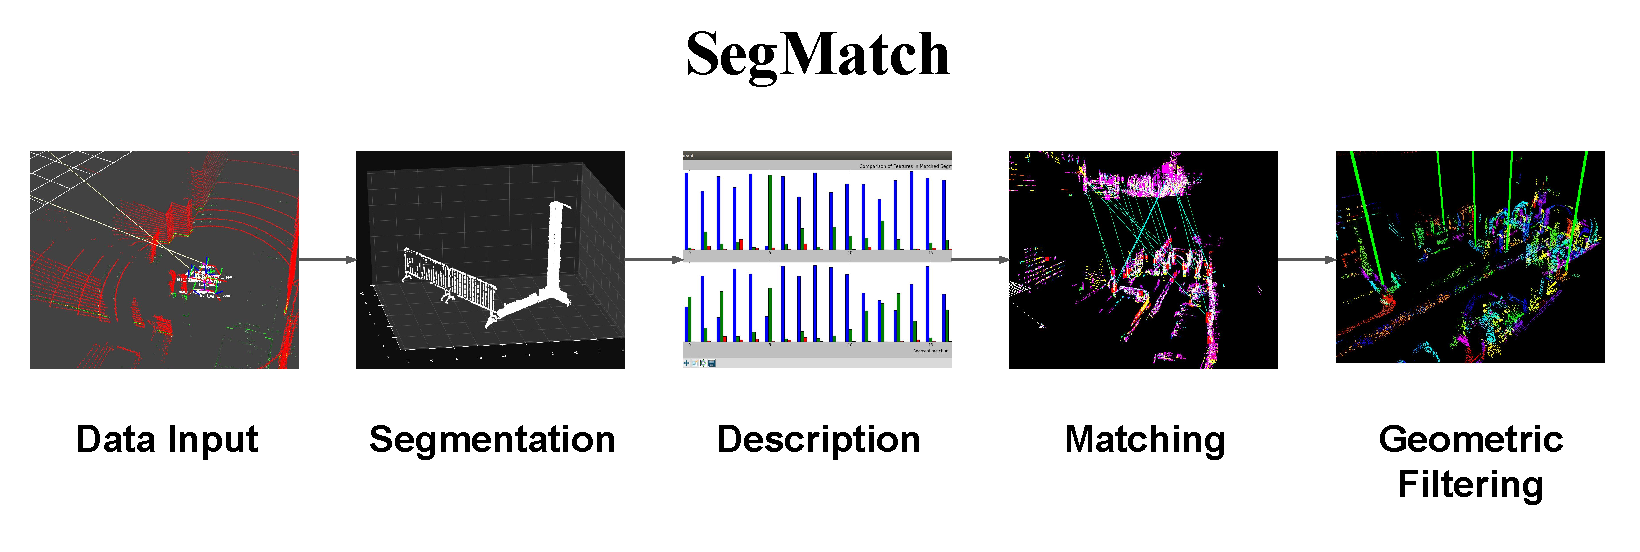
\includegraphics[width=5.2in]{images/pipeline.pdf}
  \caption{The SegMatch pipeline}
  \label{fig:pipeline}
\end{figure}

SegMatch can be used in a variety of situations where place recognition from range data is useful. Though the usual SegMatch algorithm (Fig.~\ref{fig:pipeline}) remains applicable to all such situations, there can be differences in how SegMatch should be integrated to the general pipeline, to interact with other robots or computer processes. Examples pipelines are given in Figures~\ref{fig:online_pipeline}, ~\ref{fig:offline_pipeline}, and ~\ref{fig:multirobot_pipeline} to showcase various uses of the SegMatch algorithm.\\

\begin{figure}
  \centering
  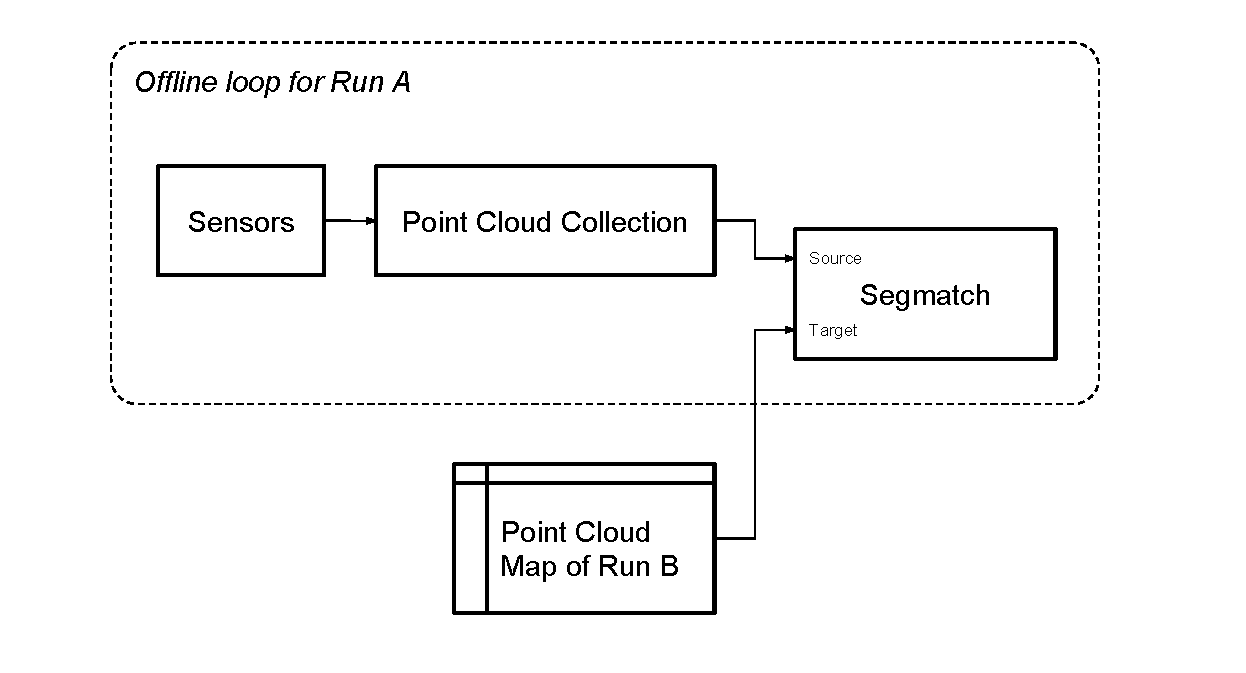
\includegraphics[width=5.2in]{images/Offline_Pipeline.pdf}
  \caption{SegMatch pipeline example: Offline matching. In this scenario, a sensor recording, in simulated time, is matched against a pre-mapped environment. The pre-mapped environment is extracted from a previous run.}
  \label{fig:offline_pipeline}
\end{figure}

\begin{figure}
  \centering
  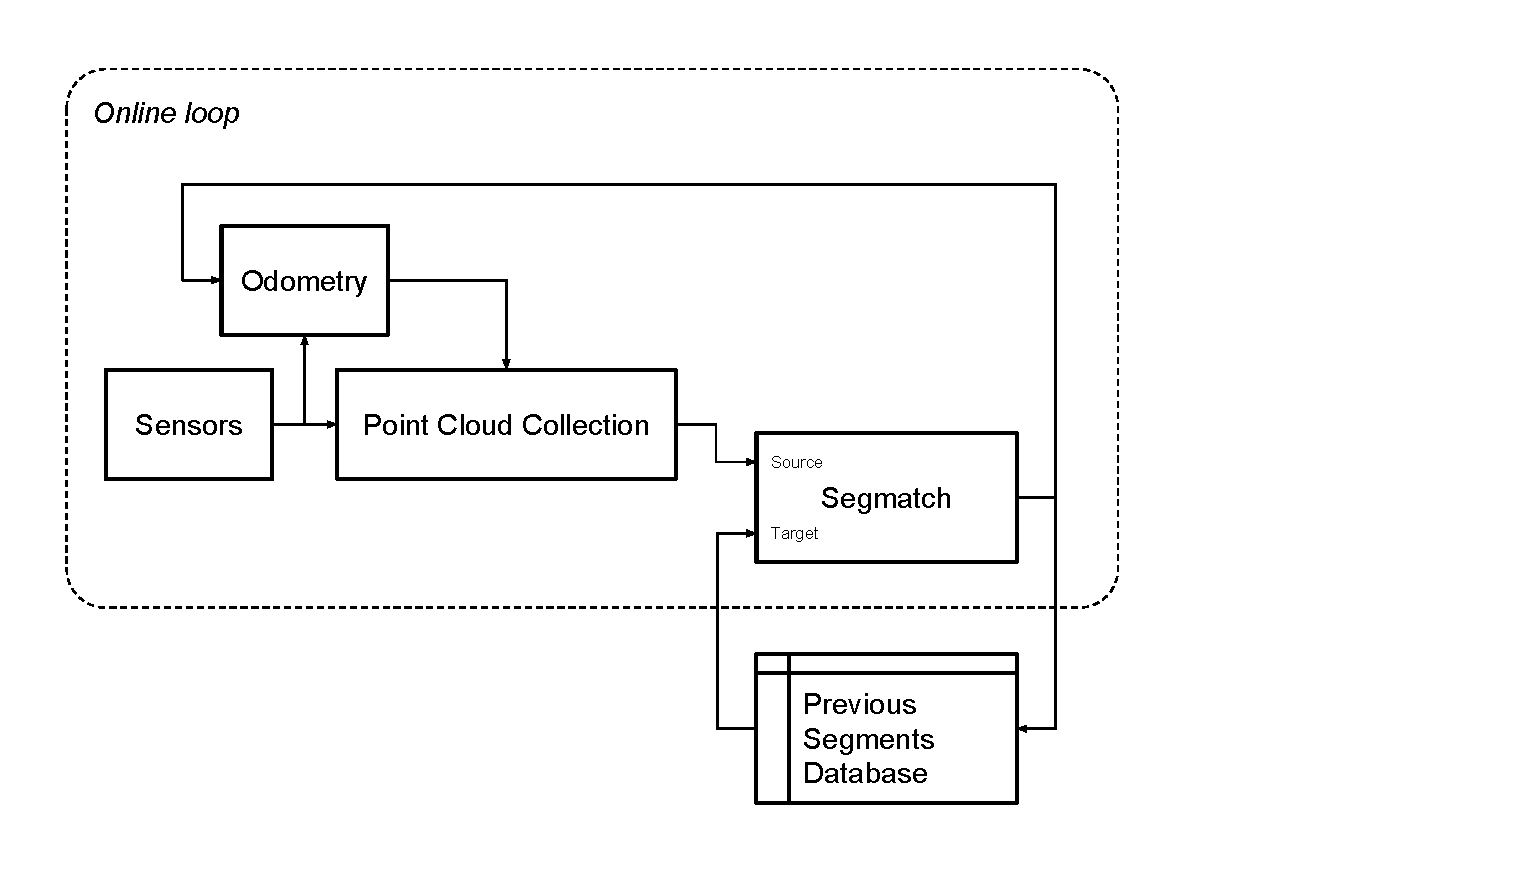
\includegraphics[width=5.2in]{images/Online_Pipeline.pdf}
  \caption{SegMatch pipeline example: Online matching. In this scenario, a single recording, or sensor stream, is fed in real-time to SegMatch. SegMatch then stores resulting segment descriptions into a database. These segments then become the "past environment", against which newer segment descriptions are matched.}
  \label{fig:online_pipeline}
\end{figure}

\begin{figure}
  \centering
  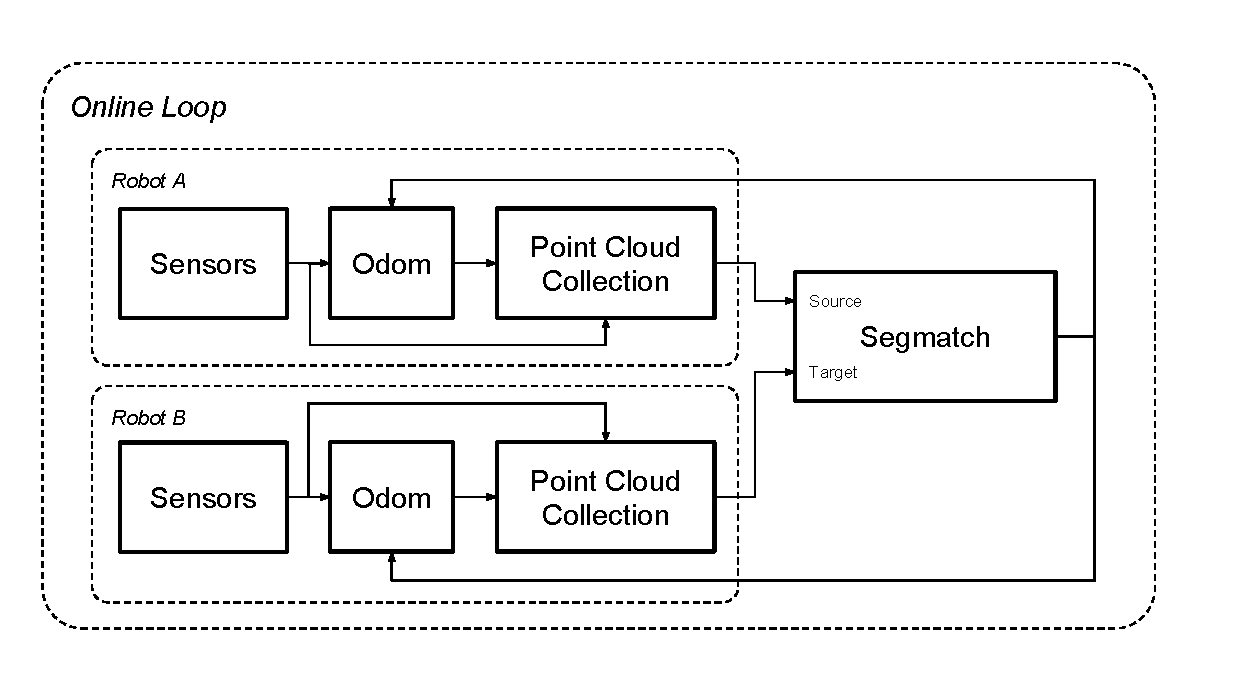
\includegraphics[width=5.2in]{images/Multi-robot_Pipeline.pdf}
  \caption{SegMatch pipeline example: Multi-robot. In this scenario, several robots explore an environment simultaneously. SegMatch is used to match between their sensor outputs, in order to detect potential positional relationships between the robots based on their surroundings. This allows the creation of a single consistent map by multiple agents.}
  \label{fig:multirobot_pipeline}
\end{figure}


\section{Input Data Pre-Processing}
\label{sec:input}

The first step of SegMatch is to acquire data on which the algorithm is performed. Usually, LiDAR sensors do not produce ready-made point clouds of the local area. In this case, this section illustrates ways in which raw sensor data can be transformed into a local map, which then becomes the input to the following step (segmentation). This pre-processing step is often run continuously in order to update the local map every time new sensor data is received. Unless the local map is deemed ready to be matched, only this pre-processing step is executed.\\


\subsection{Sensor Data}
\label{subsec:sensordata}

Two types of sensors were used in the course of this project, rotating sensors and 2D range-finder sensors with a rolling mechanism. The sensor output takes the form of a list of points, each point as a 3D coordinates and an intensity value.\\

Rotating sensors have a 360° view. With each rotation, they scan points along a cone originating from the sensor, resulting in a single circular scan line. This cone angle is varied by a set amount after each full rotation, with a maximum absolute angle making it so that the sensor is unable to scan the area directly above or under it. A typical rotating sensor scan is illustrated in Fig.~\ref{fig:velodyne-scan}. The sensor itself is pictured in Fig.~\ref{fig:velodyne}.\\

2D range-finding sensors have an approximate 180° view, scanning towards the front and sides. The scan is flat, meaning that the points are all located on the same plane relative to the sensor’s roll angle. By varying this roll angle mechanically with every subsequent scan, the sensor can produce points at many vertical angles towards its sides. A 2D range-finding sensor is pictured in Fig.~\ref{fig:sick}\\


\begin{figure}
  \centering
  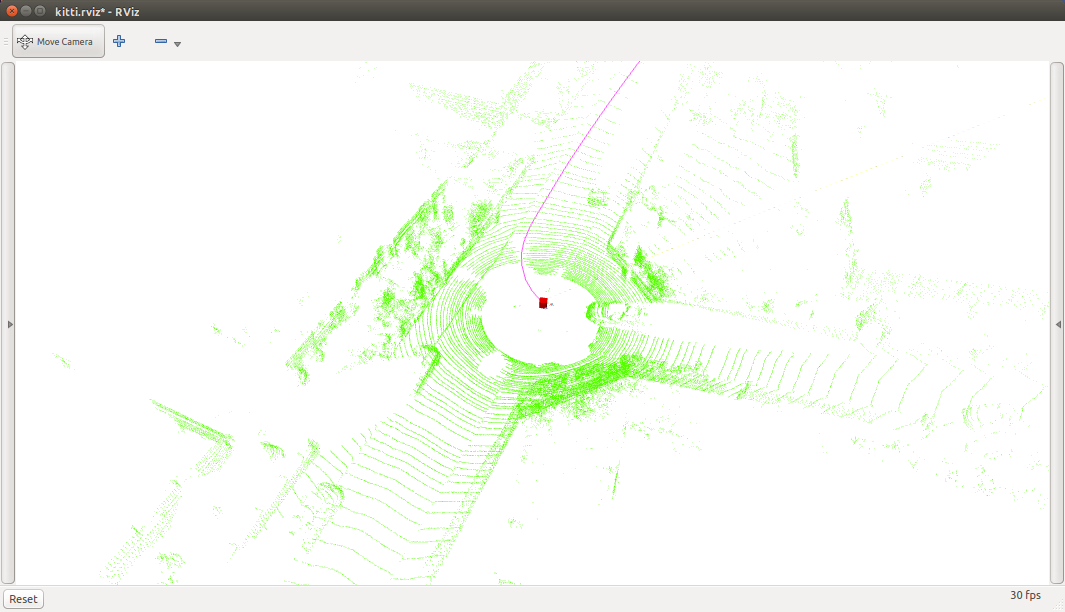
\includegraphics[width=3.2in]{images/1_velodyne_scan.png}
  \caption{Typical output of a single 360 \degree scan created by a LiDAR sensor of the rotating type, such as the sensor pictured in Fig~\ref{fig:velodyne}.}
  \label{fig:velodyne-scan}
\end{figure}

\begin{figure}
  \centering
  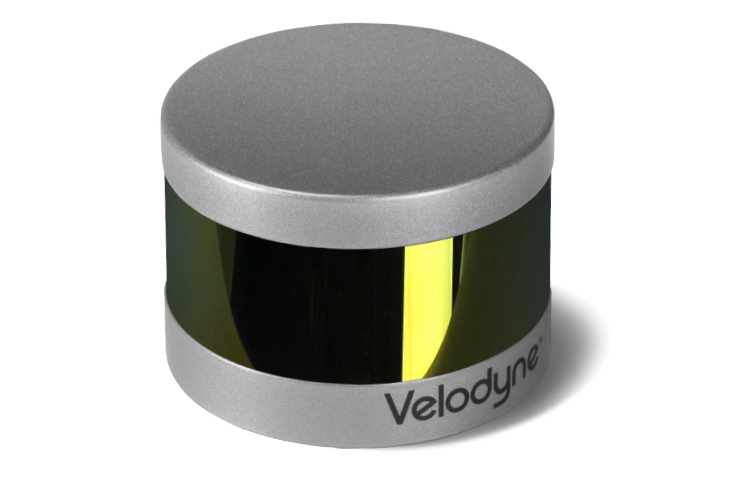
\includegraphics[width=3.2in]{images/Velodyne.png}
  \caption{A rotating LiDAR sensor, manufactured by Velodyne.}
  \label{fig:velodyne}
\end{figure}

\begin{figure}
  \centering
  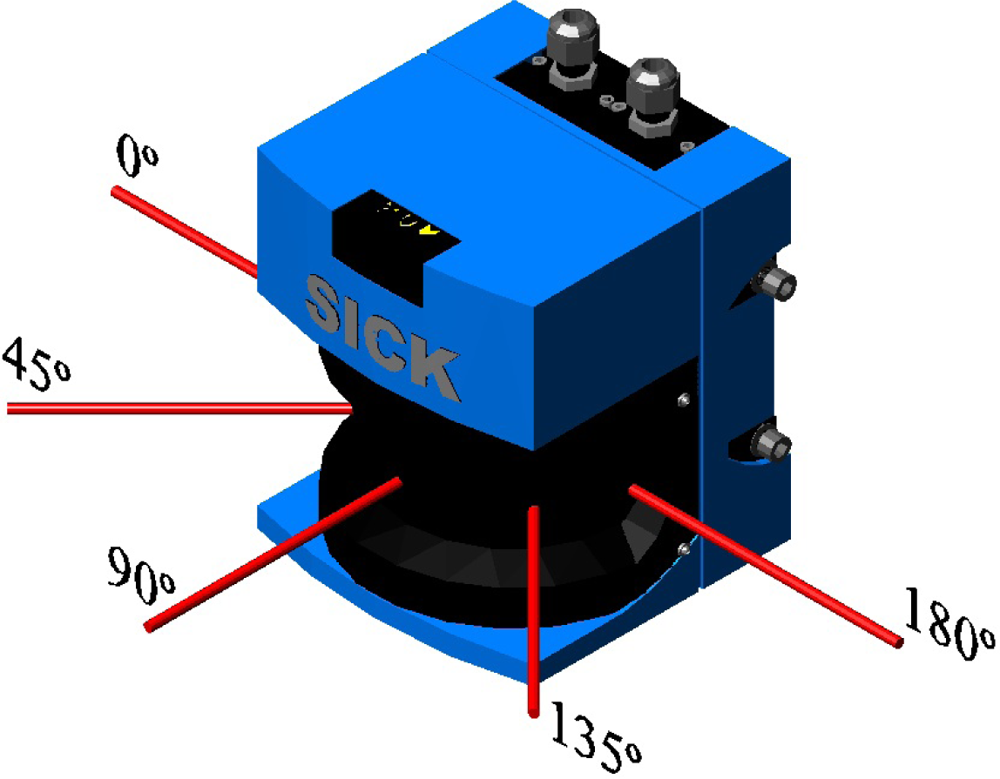
\includegraphics[width=3.2in]{images/SICK.png}
  \caption{A 2D range-finder LiDAR sensor, manufactured by SICK.}
  \label{fig:sick}
\end{figure}

\subsection{Data Distortion}
\label{subsec:distortion}

As the sensor scans its surroundings, the robot may move and rotate. An extremum example: should the robot counter-rotate at the same angular velocity as its rotating-scanner, all points will be located on the same vertical plane in the world frame.\\

Naively mapping the full scan from sensor frame to world frame with a single affine transform will not accurately portray this effect. This is because each point is taken at a different moment in time, and thus each has its own frame relative to the world frame - should the sensor be continually moving.\\

Precise knowledge of the robot’s odometry at various times during the scanning process allows to correct for distortion, by associating a different affine mapping from sensor frame to world frame to each group of points taken at a discrete rotation angle of the sensor.\\

In the case of rotating sensors: in order to correct the distortion in the aforementioned manner, we use the velodyne-assembler package created by Philipp Kruesi.

\subsection{Sensor Artefacts}
\label{subsec:artefacts}

After being corrected for distortion, sensor data contains registration patterns, as visible in Fig.~\ref{fig:velodyne-scan} (in this case, scan lines due to the rotating sensor's registration mechanics).

\subsection{Laser SLAM}
\label{subsec:SLAM}

As single sensor scans contain registration patterns (Subsection ~\ref{subsec:artefacts}), subsequent scans should be accumulated while the robot and sensor move, in order to collect data over the whole environment. Should the scans be assembled correctly, i.e, according to the correct transform w.r.t. each other, registration patterns get progressively reduced, as the accumulated data densifies.\\

To do so, knowledge of the robot's position and orientation at each sensor acquisition time is required. When the robot odometry is not sufficiently trustworthy, the Laser SLAM algorithm allows using the sensor data to increase the odometry knowledge and improve the quality of the accumulated data.\\

This algorithm corrects the odometry by registering the new scans with the map using Iterative Closest Point (ICP). The laser and odometry measurements are finally combined using a pose-graph relaxation approach. The output is a 3D point cloud which becomes the input to the next step.

\section{Segmentation}
\label{sec:segmentation}

The process of segmentation consists in clustering points which share a common property. In our case, the goal is for that property to be appartenance to a particular object, in the real-world space equivalent to point-cloud space.\\

The input of this step is a 3D point cloud. If both source and target clouds are to be segmented, this step is simply applied once to the source and once to the target, in exactly the same way.\\

An ideal segmentation target is however not explicitly defined. Should the point-cloud of a building be segmented into more basic components, such as walls, windows, and doors, or as single large cluster? Should a tree be clustered as a trunk with clusters of leaves above it or as a single cluster (illustrated in Fig.~\ref{fig:hierarchical})?\\

Moosman \cite{moosmann2011unsupervised} proposes to hierarchically segment the scene, i.e., to cluster point clouds into not only segments, but also subsegments and subsubsegments. As a result, a single point can be assigned to a segment, \textit{and} one of its subsegments, and so on. This segment hierarchy is established in order to capture those patterns that exist in real-world objects, which can be composed of smaller, simpler objects.\\

\begin{figure}
  \centering
  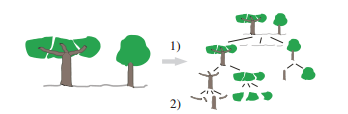
\includegraphics[width=3.2in]{images/hierarchical.png}
  \caption{Illustration of the hierarchical segmentation concept, by Moosman \cite{moosmann2011unsupervised}}
  \label{fig:hierarchical}
\end{figure}

It is useful to be aware of this concept of segment hierarchy even when using straightforward segmentation methods. \textit{Straightforward}, in this context, refers to segmentation algorithms which assign each point to at most one segment, and do not consider sub-, subsub- segments, and so on. Awareness of this hierarchy allows us to evaluate the output of our segmentation algorithm w.r.t. where it lies on this hierarchy, and how that relates to the usefulness of the segments it produces. To illustrate, a specific algorithm, using a certain set of parameters, could tend to find segments which are very low in the hierarchy, i.e, smaller, less complex segments. This gives us a larger number of less unique segments, than say, running the same algorithm at a different scale.  
By understanding this, it is easier to select the parameters which lead to optimal size, number and complexity of segments for the purposes of one's own use-case.\\

In this section, we present the main segmentation algorithms implemented and used in SegMatch. Their output and performance is discussed.  
It should be noted that other segmentation algorithms exist and are not presented here.\\

\subsection{Euclidean Clustering}
\label{subsec:euclidean}
%TODO

Euclidean clustering is the simplest segmentation method presented here. It consists in clustering together points which fall below a certain distance threshold $\delta$ from each other. This threshold is the only parameter of the algorithm.\\

It is outlined by Douillard et Al. \cite{douillard2011segmentation} as the 'Cluster-All Method' of segmentation.\\

In terms of performance, the algorithm is very fast, allowing SegMatch to perform segmentation in real-time even on the fastest moving KITTI \cite{KITTI} datasets. This is due to the algorithm's simplicity.\\

On the other hand, large objects are often segmented as single clusters, and smaller objects are often clustered together simply because they happen to lie close to each other.\\

Finally, it is generally necessary to filter out the ground as it tends to connect many objects together. This can offload complexity to ground filtering in the case of complex ground geometry, but is relatively simple to do in the case of a flat city street.\\

An example output for this segmentation algorithm, after filtering the ground-plane is illustrated in Fig.~\ref{fig:euclidean-segments}.

\begin{figure}
  \centering
  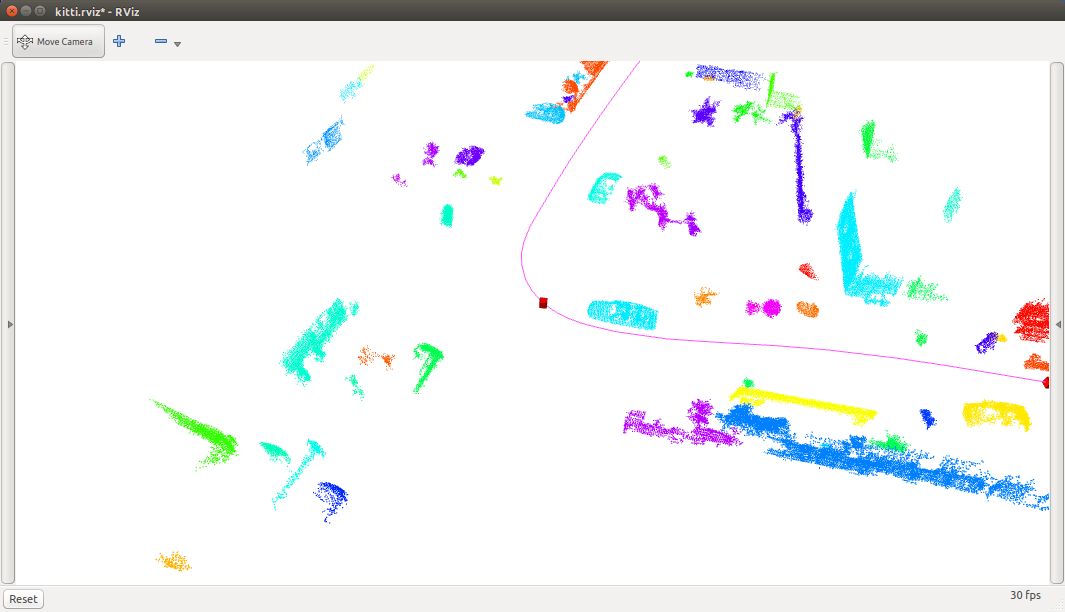
\includegraphics[width=3.2in]{images/3_segments.png}
  \caption{Example of segments extracted with the euclidean segmentation algorithm, after filtering the ground plane. The car segments near the middle of the figure are very distinct and useful segments. Also visible are single large segments of buildings (middle-right), and single segments fusing together several objects (trees and facades, bottom right).}
  \label{fig:euclidean-segments}
\end{figure}

\subsection{Difference of Normals Segmentation}
\label{subsec:DoN}
%TODO

Ioannou \cite{ioannou2012difference} presents the Difference of Normals segmentation algorithm, which aims to filter out geometrically uninteresting sections of the environment.  
In order to do this, a difference of normals operator is defined, describing the variation in orientation with respect to scale, in the neighbouring environment. An illustration of this operator is shown in Fig.~\ref{fig:DoN}.\\

\begin{figure}
  \centering
  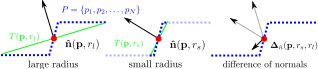
\includegraphics[width=3.2in]{images/DoN.png}
  \caption{The DoN operator proposed by Ioannou \cite{ioannou2012difference}}
  \label{fig:DoN}
\end{figure}

The normals are first calculated at each point considering a neighbourhood of radius $r_l$, the large scale radius, then again for neighbourhood of radius $r_s$, the small scale radius. This process is often computationally heavy, increasingly so as the large scale increases (if nearest neighbours are not subsampled).\\

For each point, a difference of normals $\Delta_n$ is calculated between the average neighbour normals for the two scales. As a result, areas which are flat at both the large and small scale have a low difference of normals. Those points are filtered out according to the threshold $\Delta_n > \Delta_n^{threshold}$, and the remaining points are clustered together if their DoN operators are similar.\\

Parameters for this algorithm are $r_s$, $r_l$, $\Delta_n^{threshold}$. An example output for this segmentation algorithm is illustrated in Fig.~\ref{fig:don-segments}.\\

\begin{figure}
  \centering
  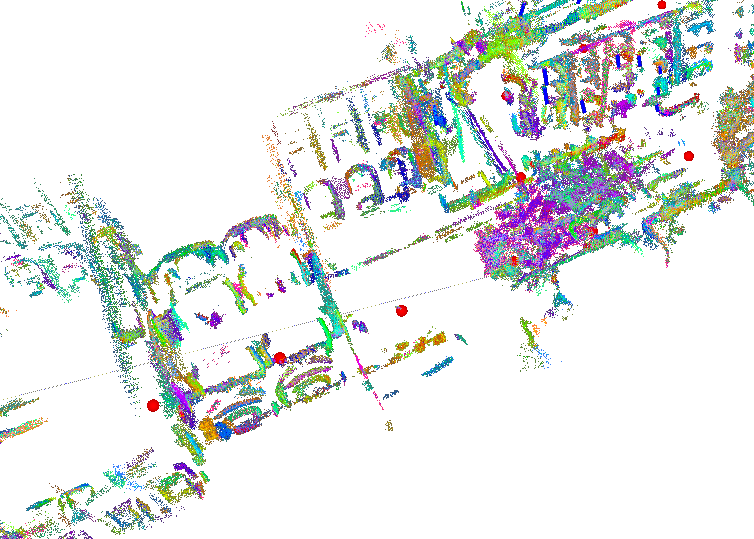
\includegraphics[width=3.2in]{images/don_segments.png}
  \caption{Example of segments extracted with the DoN segmentation algorithm. As visible in the figure, this algorithm allows the extraction of many distinctive component segments from single large objects, such as window frames, arches, and small facades.}
  \label{fig:don-segments}
\end{figure}

\section{Description}
\label{sec:description}

Descriptors allow us to compress information about each segment's properties into an n-dimensional feature vector, which offers a suitable signature for matching.\\

The input to this step is a list of segments. The output is a n-dimensional feature vector, a \textit{description}, for each segment. Like the segmentation step, this step is applied once to source and once to target data.\\

An ideal descriptor would yield identical feature vectors for any segments which are views of the same real-world object. If two segments represent views of different objects their feature vectors should differ.  
In other words, ideal descriptors lead to strong clustering in the n-dimensional feature space of segments representing views of the same objects. \\

A good descriptor is a descriptor which approaches this behavior, where segments which are views of the same object are often clustered close to each other. Weaker clustering in accordance with object classes (objects that are similar yet not identical) can reasonably be expected.\\

This section outlines the pre-existing segment description algorithms used in SegMatch. In Chapter \ref{chap:ae}, we introduce our own descriptor based on an unsupervised learning approach.\\

The list of descriptors presented in this section is in no way exhaustive.\\

\subsection{Eigenvalue-based Features}
\label{subsec:eigenvalues}

Eigenvalue based features are proposed in Weinmann \cite{weinmann2014semantic}. This descriptor yields 7 feature values:

\begin{itemize}
  \item{Linearity = $\frac{\lambda_1 - \lambda_2}{\lambda_1}$}
  \item{Planarity = $\frac{\lambda_2 - \lambda_3}{\lambda_1}$}
  \item{Scattering = $\frac{\lambda_3}{\lambda_1}$}
  \item{Omnivariance = $\sqrt[3]{\lambda_1 \lambda_2 \lambda_1}$}
  \item{Anisotropy = $\frac{\lambda_1 - \lambda_3}{\lambda_1}$}
  \item{Eigenentropy = $\sum\limits_{i=1}^3 \lambda_i \ln{\lambda_i}$}
  \item{Change of Curvature = $\frac{\lambda_3}{\lambda_1 + \lambda_2 + \lambda_3}$}
\end{itemize}

where $\lambda_1$, $\lambda_2$, $\lambda_3$ are the normalized eigenvalues of the covariance matrix $\mathbf{C} \in \mathbb{R}^{3x3}$
$$
\mathbf{C} = 
\begin{bmatrix}
  cov(\textbf{x},\textbf{x}) & cov(\textbf{y},\textbf{x}) & cov(\textbf{z},\textbf{x})  \\
  cov(\textbf{x},\textbf{y}) & cov(\textbf{y},\textbf{y}) & cov(\textbf{z},\textbf{y})  \\
  cov(\textbf{x},\textbf{z}) & cov(\textbf{y},\textbf{z}) & cov(\textbf{z},\textbf{z})  \\
\end{bmatrix} 
$$
$\textbf{x}$, $\textbf{y}$, $\textbf{z}$ being the coordinates of all points inside the segment.

\subsection{Ensemble of Shapes}
\label{subsec:ensemble-of-shapes}

This descriptor calculates the statistical measure of some properties for randomly selected point pairs/triplets within the object.\\

The resulting feature of dimension 1x640 is made of 10 histograms which encode the shape functions D2, D3 and A3 as described in \citet{wohlkinger2011ensemble}.
%
The D2 shape function is a histogram of the distances between randomly selected point pairs while D3 encodes the area between randomly selected point triplets.
%
The A3 shape function describes the angles between two lines which are obtained from these triplets. These shape functions are illustrated in Fig.~\ref{fig:eos}.

\begin{figure}
  \centering
  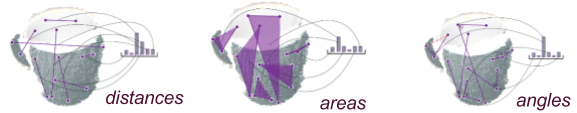
\includegraphics[width=3.2in]{images/eos.png}
  \caption{The \textit{Ensemble of Shapes} shape-functions, illustrated.}
  \label{fig:eos}
\end{figure}

\section{Matching}
\label{sec:matching}

Once descriptions of all source and target segments have been computed, the matching step is responsible for finding potential pairwise matches between source and target segments.\\ 

The inputs are one list of source segment descriptions, and one list of target segment descriptions. This step then outputs a list of potential matches between source and target segments based on their descriptions, which is processed in the next step (Geometric Consistency) in order to find potential loop closures.\\

\subsection{kNN}
\label{subsec:kNN}

The simplest matching algorithm considered here, kNN selects the k nearest neighbours according to Euclidean distances of a segment description in n-dimensional feature space.\\

In the case of an ideal descriptor, this algorithm is sufficient to recognize true segment matches, even with $k = 1$. As we recall, an ideal descriptor would ensure that all segments taken from a single object in the real world have identical features.\\ 

For sufficiently good descriptors, this algorithm can also be adequate, predicting mostly true matches and some false matches. One issue with descriptors that are not ideal is that they might not allow to distinguish precisely between objects in the same class.  
That is, segments representing cars might be clustered together, with small variation in their descriptors being tied to viewpoints or the area of a car that the segment covers, rather than distinctive characteristics in the cars themselves. In this case it can be useful to increase the value of $k$.\\

A common alternative to limiting the number of nearest neighbours with a threshold k, is to limit the nearest neighbours to all that fall within a certain threshold radius $r$. Furthermore, both thresholds can be combined, in order to limit nearest neighbours in both amount and distance.\\

It should be mentioned that descriptors do not necessarily encode features homogenously in n-dimensional space. That is, within some regions of n-dimensional space, tiny differences in description vectors might translate to large differences in the properties of described objects, while in other regions the opposite holds. Another way of phrasing this, is that the density of clusters varies in n-dimensional space. In those cases, distance in n-dimensional space does not generalize well as a measure of similarity. To illustrate, the same threshold radius can be very strict (i.e., containing many neighbours however dissimilar) in some regions of n-dimensional space, and not strict at all (i.e., filtering out all neighbours including desired ones) in others. This renders kNN methods which use a constant radius $r$ less effective.\\

For descriptors which are further from the ideal, better matching results can be obtained by using a more complex matching algorithm than kNN, as illustrated in the next section.

\subsection{Random Forests}
\label{subsec:RF}

A Random Forest is a machine learning algorithm which trains many decision trees simultaneously, then polls them in order to classify input as discussed in \cite{breiman2001random}.\\

In our case, the input is the difference between the feature vectors of two segments, and the output a boolean describing whether or not those segments are a match. This output can also instead be a probability of match $p$, with $0 \leq p \leq 1$.\\

In order to generate its decision trees, the Random Forest is presented with training examples consisting of inputs and a ground-truth output probability (In our case, two segment descriptions, and the known-in-advance probability that they are a match), and decision trees are "grown" based on these examples. During training, the randomly generated trees only have access to a subset of examples, and a subset of input values. The former allows for different trees to be "grown", while the later allows for selection of features which are useful in making correct predictions.\\

Though the Random Forest algorithm allows for much more complex selection of potential matches based on their description, it requires supervised training in order to create the necessary decision trees. This is an issue, as we have no simple solution for generating a large dataset of matching segments, and ensuring that we do not accidentally label a positive match as negative is a complex process.\\

\section{Geometric Consistency}
\label{sec:filtering}

An efficient method to extract patterns of matches from a list of potential matches is the \textit{Geometric Consistency} algorithm, based on random sample consensus (RANSAC, as presented in \citet{fischler1981random}).\\

In this algorithm, matches are clustered together if they can form an Euclidean transformation, within a spatial tolerance $r$. As the Euclidean transformation has 6 degrees of freedom, any clusters with less than 3 matches is filtered out.\\

The clusters which remain, those consisting of 3 or more matches, are loop closure candidates. The algorithm also returns the transformations formed by each of these clusters. A stricter ($>3$) threshold on the minimum number of matches in clusters can be set to increase robustness. In the case where several loop closure candidates are found, but a single one is desired, the one corresponding to the largest cluster of matches is selected.\\

\section{Applying SegMatch - Online Example}
\label{sec:online}

Thus far into this chapter, the usual steps of the SegMatch algorithm have been presented. SegMatch can be applied to several situations, as outlined in Section \ref{sec:intro-pipeline}, without needing to modify any of the steps in the above sections.\\

What does change between implementations is \textit{when} to run SegMatch, \textit{what data} is to be taken as input, and of course the parameters.\\

The present section illustrates an example of how we applied SegMatch, in the case of a full online loop-closure-detection module with a ROS interface.

\subsection{Segmentation Strategy}
\label{subsec:segmentation-strategy}

In the online scenario, the goal is to use SegMatch as-we-go in order to attempt to find matches between the most recent section of the environment, and the recorded past environment.\\

Our pipeline for this scenario is illustrated in Fig.~\ref{fig:online_pipeline}. It is explained in detail as follows:

\begin{enumerate}
  \item Odometry and LiDAR sensor data is continually fed to the pre-processing step, which uses both the odometry and LiDAR scans to accumulate a map (as explained in Subsection \ref{subsec:SLAM}). No other steps are performed until the map is deemed ready to be matched. This continually updated map is the source map.
  \item When the robot has moved 20 meters away from the previous SegMatch position (experimental and theoretical reasons behind this are discussed in \ref{subsec:segmentation-frequency}), SegMatch is applied between this source map and the target map (initially empty).
\item At the end of the SegMatch iteration, the descriptions of segments extracted from the source map are added to the target map. The source map is cleared, and the process begins anew with step 1.
\end{enumerate}


\begin{figure}
  \centering
  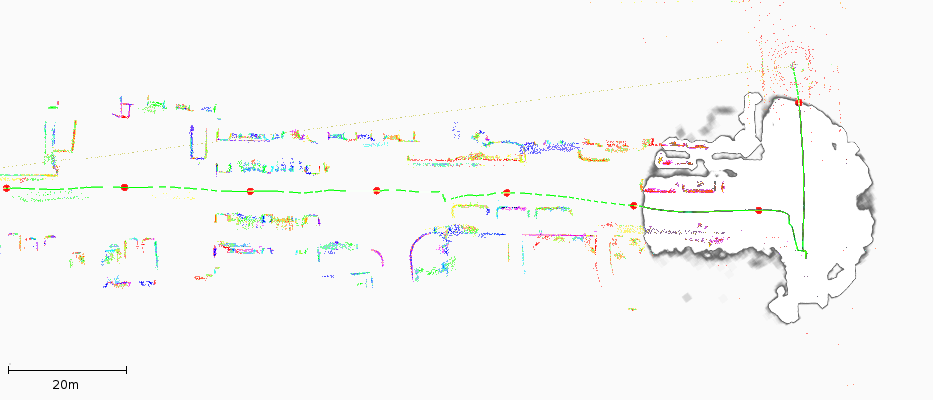
\includegraphics[width=5.2in]{images/seg_queue.png}
  \caption{A top-down view of the online segmentation process. In green, as a thin curve, is the robot trajectory. The trajectory runs from left to right, and thus at the top right end of this curve is the latest robot position. Around this point the latest Velodyne scan is faintly visible in red. Red spheres visible placed along the trajectory mark the past robot locations at which SegMatch was applied. Visible shapes surrounding this trajectory are segments stored in the target map. These segments are given arbitrary colors to visually distinguish them. The circular area at the right delimitates the latest local map, which is about to be segmented and matched against the target.}
  \label{fig:seg-queue}
\end{figure}

Fig.~\ref{fig:seg-queue} illustrates the process of online segmentation described above.


\subsection{Filtering Segments}
\label{subsec:filtering-segments}

Based on the range of the velodyne sensor, density of the local map decreases as distance from the sensor increases. Thus, regions far from the sensor have low density, with associated registration patterns. For this reason, we have found that it is beneficial to apply a cylindrical filter at each segmentation position, with a max radius $R$. All points from the local map situated outside of $R$ are erased. This results in the distinct circular shape of the local map in Fig.~\ref{fig:seg-queue}.\\

It makes sense for this radius to be larger than the distance between SegMatch positions, as some areas along the robot trajectory would otherwise be ignored. However, this leads to overlap between subsequent local maps.

\subsubsection{Duplicates}
\label{subsub:sec:duplicates}

Duplicate segments occur due to overlap between subsequent local maps, or when revisiting a section of the environment.
In our experiments, results indicate that it is necessary to prevent duplicate segments from being stored, as they later create duplicate matches.\\ 

These duplicate matches are detrimental to the Geometrical Clustering step, either artificially increasing the amount of matches in a cluster, or even creating clusters consisting only of identical matches (with an exaggerated transformation, since there is not enough true degree of freedom information in those duplicate matches) which favorizes false loop closures.\\

In order to identify duplicate segments, we look at segments who are mutual nearest neighbours, and which are within a small distance $d_{duplicate}$ from each other. Distances between segments are calculated w.r.t. the segments centroids. We set the value of the $d_{duplicate}$ parameter to 1m, determined empirically. When duplicates are detected, the newest segment is kept, and older duplicates are deleted.\\

\subsubsection{Partial Segments}
\label{subsubsec:partial}

In the case where the SegMatch algorithm is applied to point clouds which have had a boundary filter applied, it is common for segments lying close to the boundary to be partial views of objects which lie on the boundary. 
These partial segments can lower the quality of the matches and the general algorithm performance, as such it is recommended to find and eliminate such partial segments. 
In order to do so, our method consists in first segmenting the boundary filtered point cloud, then applying a stricter version of the same boundary filter.\\

For example, say that the boundary filter is cylindrical of radius $R$. We consider a cylinder of smaller radius $r = R-b$, $b$ being the thickness of the 'outer zone'. Segments that have points within this 'outer zone' are considered to likely also possess points outside of $R$, and therefore to be partial segments. Thus, they are removed. We use a value of 2m for $b$, determined empirically.\\


\section{Results}
\label{sec:segmatch-results}

% \subsection{Influence of parameters}
% This subsection evaluates the influence of algorithm parameters on the output.\\
%TODO

\subsection{Loop closures}

We now demonstrate the loop closure capabilities of SegMatch, which were achieved with minimal parameter tuning.\\

SegMatch was tested on the public KITTI odometry dataset (drive 18, 20, 27), as well as in real-world experiments. On all datasets as well as in our experiments, SegMatch was able to identify useful loop closures, and correct previous trajectory errors accordingly. Over a large amount of trials, the ratio of false-to-true loop closures was measured to be below 3\%.\\

Dubé \cite{segmatch}, the scientific publication which issued from this work, presents a comparison between SegMatch and Keypoint-based methods (see Fig.~\ref{fig:segmatch-vs-keypoints}), as well as statistics for SegMatch offline loop-closure finding capabilities. Both show promising results for the SegMatch algorithm.\\

\begin{figure}
  \centering
  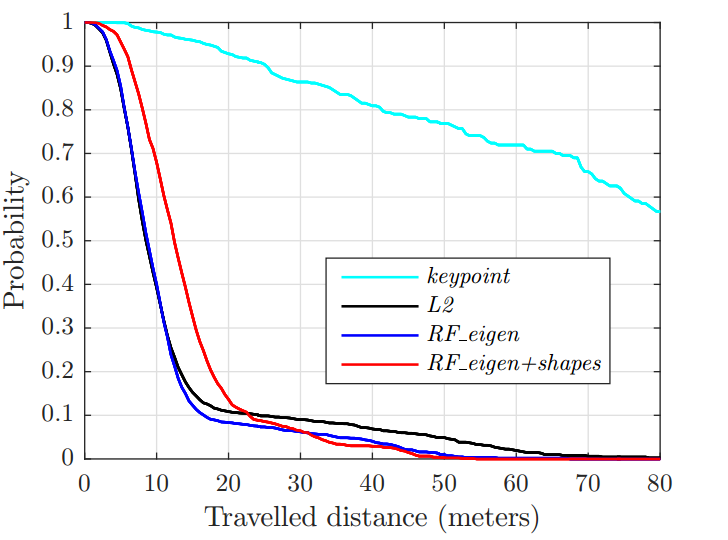
\includegraphics[width=3.2in]{images/segmatch_vs_keypoints.png}
  \caption{Probability of travelling a given distance before localizing in the target segment map. Data is obtained from 90 localization runs for each strategy on drive 00 of the KITTI  dataset. \textit{L2}, \textit{RF\_eigen}, and \textit{RF\_eigen+shapes} refer to variants of the SegMatch algorithm using respectively eigenvalue-based description with kNN+threshold matching, eigenvalue-based description with Random Forest matching, and eigenvalue-based + ensemble-of-shapes description with Random Forest matching. \textit{keypoint} refers to a keypoint method for finding loop closures, further detailed in \citet{segmatch}. Over these 90 runs, the \textit{keypoint} and \textit{L2} strategies respectively detected 292 and 14 false loop-closures while \textit{RF\_eigen} and \textit{RF\_eigen+shapes} made no false detections.}
  \label{fig:segmatch-vs-keypoints}
\end{figure}

On the KITTI dataset, the method of segmentation used was Euclidean Clustering (Subsection \ref{subsec:euclidean}). On our own dataset (named "Clausiusstrasse" after the street it was taken on), Difference of Normals segmentation was used instead, for two main reasons: 1) The scene being dominated by large objects, a segmentation yielding smaller segments was preferred. 2) Our robot NIFTI moves at human walking speed, therefore much slower than KITTI's cars. This slow movement allows for enough processing time to perform Difference of Normals calculations in real-time.\\
%TODO

\begin{figure}
  \centering
  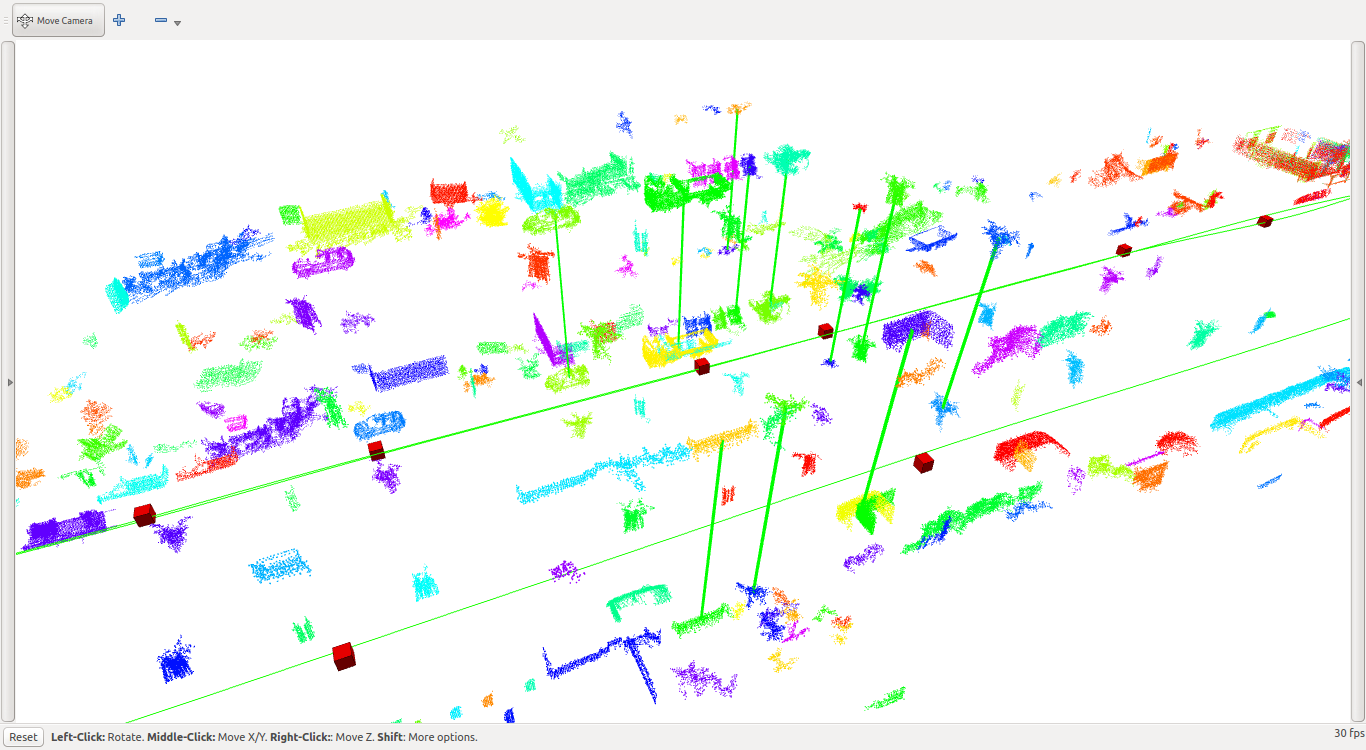
\includegraphics[width=5.2in]{images/segmatchae.png}
  \caption{Example of a successful SegMatch online loop closure detection on KITTI drive 20. As in Fig.~\ref{fig:seg-queue}, the robot trajectory is represented as a thin green curve, with red markers indicating past SegMatch locations, and arbitrary color-coded segments. For visualization purposes, the source segments are virtually raised by 15 meters above the target segments. This allows the matches between segments, detected by SegMatch, to be shown as green vertical lines.}
  \label{fig:segmatch-loop-closure}
\end{figure}

\begin{figure}
  \centering
  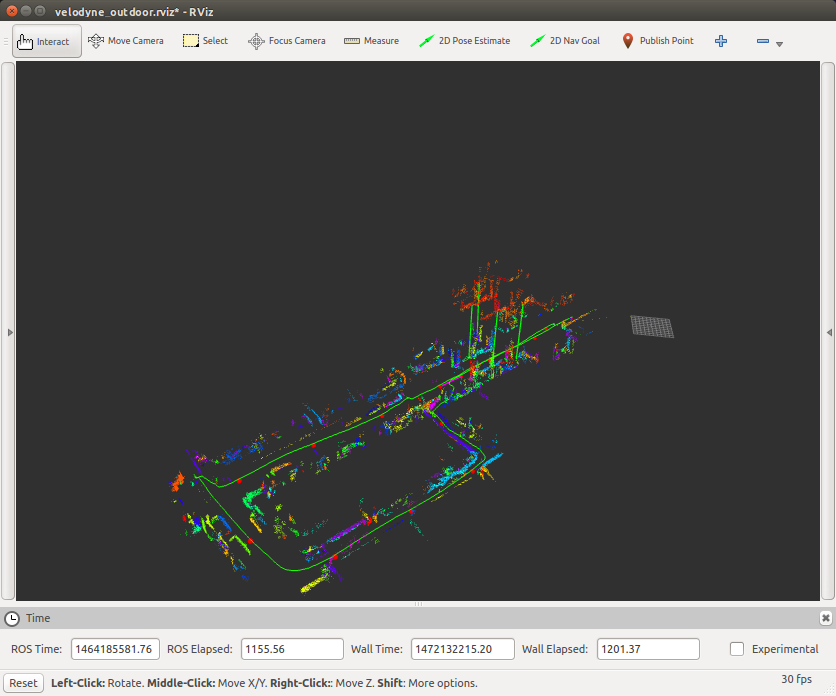
\includegraphics[width=5.2in]{images/clausius2.png}
  \caption{Example of a successful SegMatch online loop closure detection during a real-world experiment on Clausiusstrasse, using a terrestrial robot with a Velodyne rotating LiDAR sensor. Robot trajectory, target and source segments, matches, and SegMatch positions are visualized using the same markers as in Fig.~\ref{fig:segmatch-loop-closure}.}
  \label{fig:clausius2}
\end{figure}

Fig.~\ref{fig:corrected} shows the final result of SegMatch being applied in real time, during a single run on KITTI drive 18. The loop closure candidates identified by our algorithm are fed into a sparse pose graph optimizer which yields a more accurate trajectory and map. In this example, drift was artificially induced into the KITTI dataset (which otherwise contains true GPS baseline).\\

\begin{figure}[!tbp]
  \centering
  \begin{minipage}[b]{0.4\textwidth}
    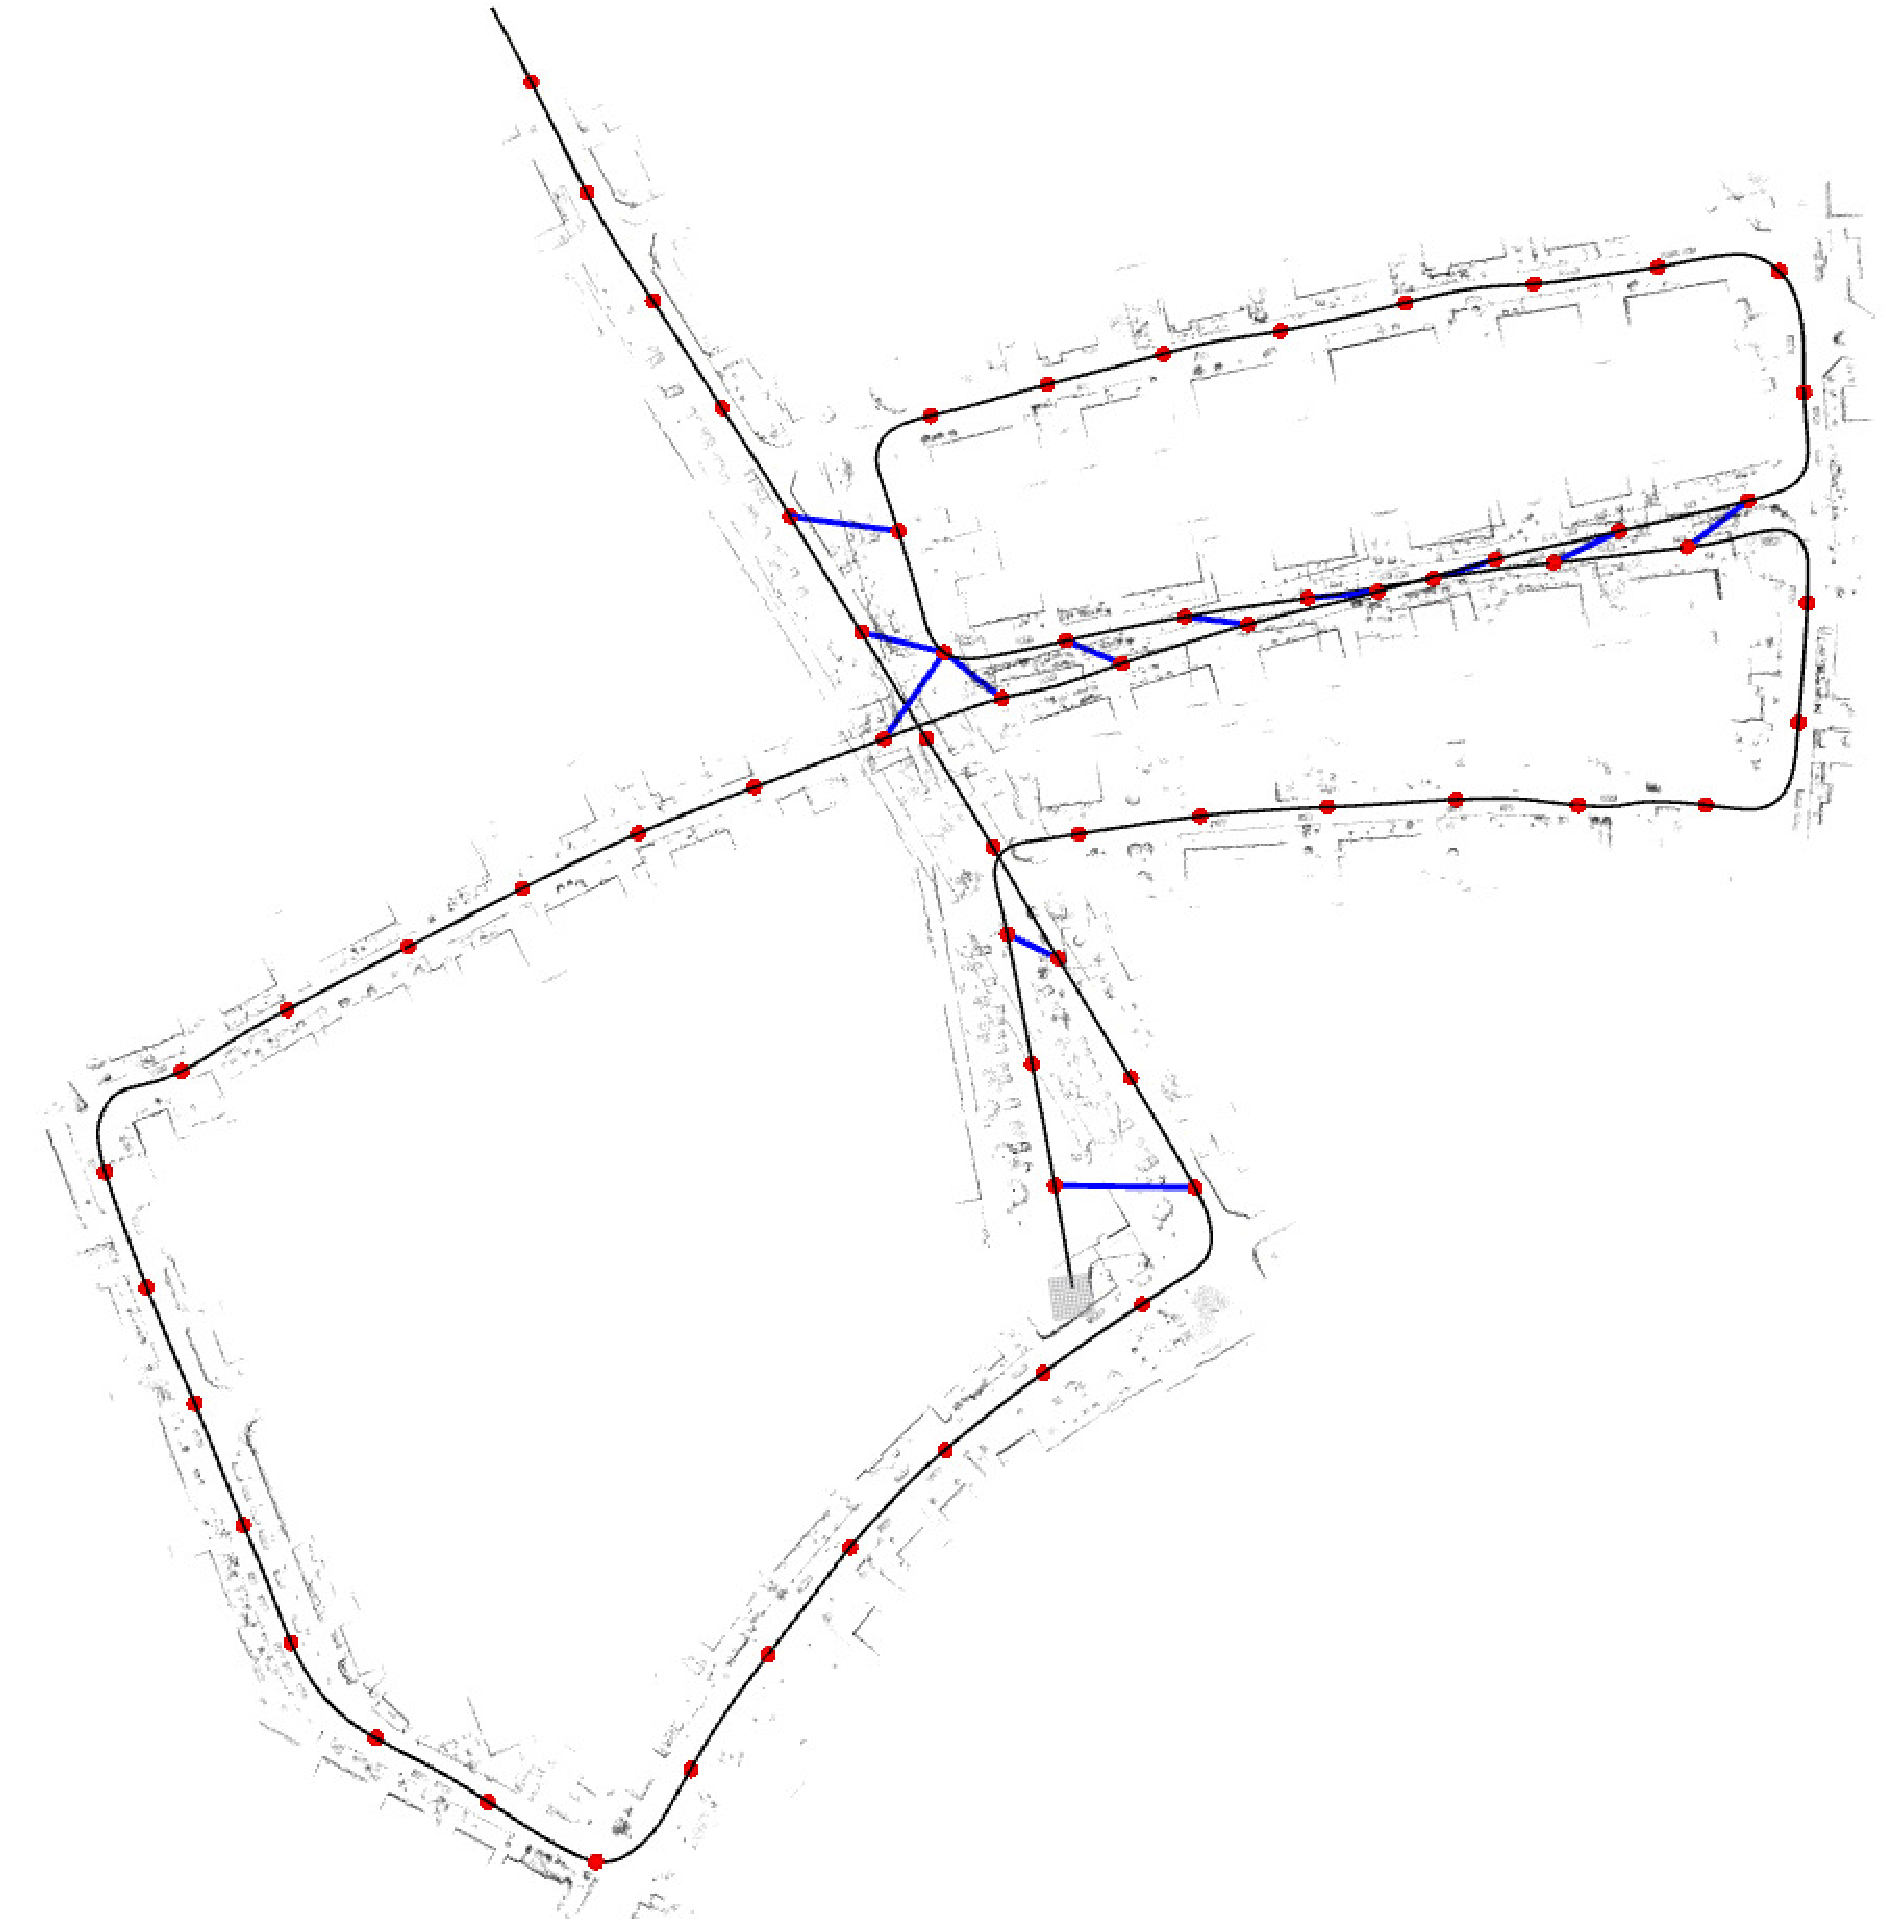
\includegraphics[width=\textwidth]{images/before_segmatch.pdf}
  \end{minipage}
  \hfill
  \begin{minipage}[b]{0.4\textwidth}
    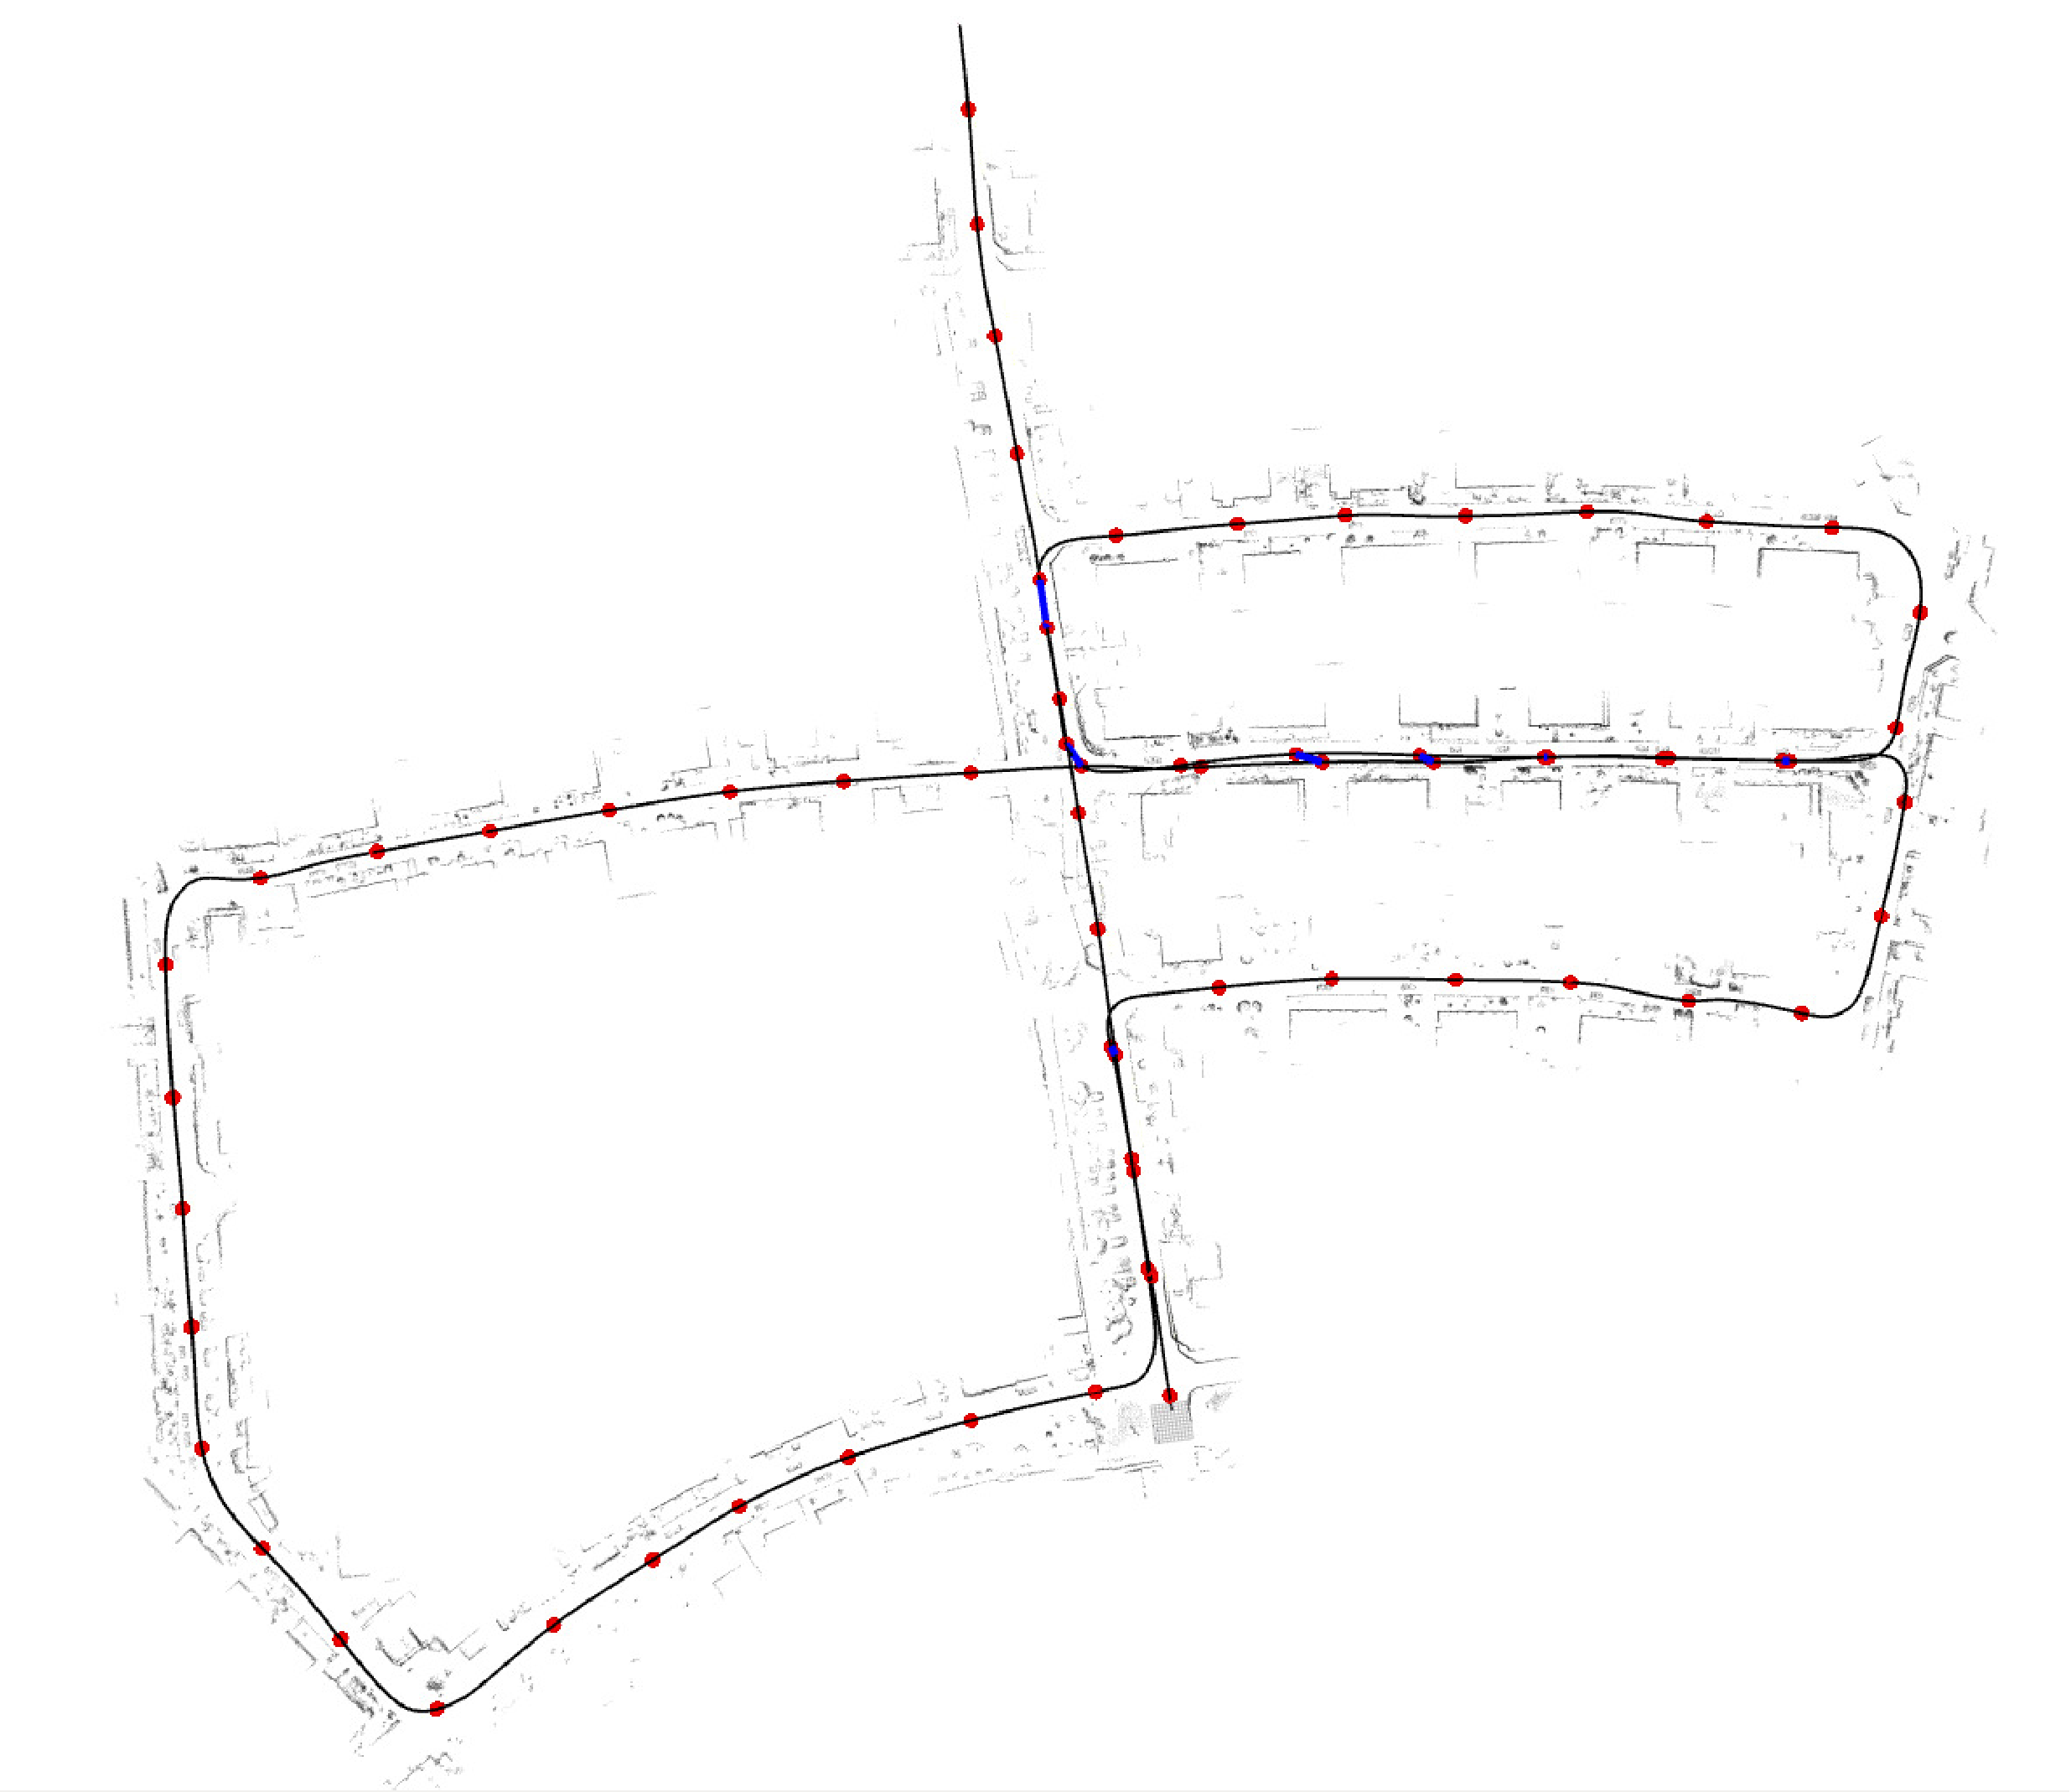
\includegraphics[width=\textwidth]{images/after_segmatch.pdf}
  \end{minipage}
  \caption{Illustration of loop-closure with \textit{SegMatch}: (a) Shows loops detected in real time by the segment based strategy \textit{RF\_eigen+shapes} during sequence 05. The red dots represent locations where segmentation and loop-closure detection were performed and the blue lines indicate the detected loops (with no false positives). (b) Illustrates the result of feeding these loops to an online pose-graph trajectory estimator.}
  \label{fig:corrected}
\end{figure}

